% !TeX TS-program = xelatex

\documentclass[aspectratio=169]{beamer}

\usepackage{xltxtra}
\usepackage[main=russian,english]{babel}
\defaultfontfeatures{Mapping=tex-text}
\usepackage{listings}

\usepackage[backend=biber,bibstyle=numeric,citestyle=numeric-comp,sorting=none,defernumbers=true,date=long]{biblatex}
\addbibresource{strangego.bib}

\makeatletter
\let\old@lstKV@SwitchCases\lstKV@SwitchCases
\def\lstKV@SwitchCases#1#2#3{}
\makeatother
\usepackage{lstlinebgrd}
\makeatletter
\let\lstKV@SwitchCases\old@lstKV@SwitchCases

\lst@Key{numbers}{none}{%
    \def\lst@PlaceNumber{\lst@linebgrd}%
    \lstKV@SwitchCases{#1}%
    {none:\\%
     left:\def\lst@PlaceNumber{\llap{\normalfont
                \lst@numberstyle{\thelstnumber}\kern\lst@numbersep}\lst@linebgrd}\\%
     right:\def\lst@PlaceNumber{\rlap{\normalfont
                \kern\linewidth \kern\lst@numbersep
                \lst@numberstyle{\thelstnumber}}\lst@linebgrd}%
    }{\PackageError{Listings}{Numbers #1 unknown}\@ehc}}
\makeatother

\setmainfont{Arial}
%\setromanfont{Times New Roman}
%\setsansfont{Arial}
%\setmonofont{Courier New}

\title{Почему Golang такой странный}
\author{Филипп Кулин (Дремучий лес)}

\usetheme{gcr2019}

\setbeamercolor{itemize item}{fg=text}
\setbeamercolor{itemize subitem}{fg=text}
\setbeamercolor{alerted text}{fg=text}
\setbeamertemplate{itemize items}{\textbullet}
\setbeamerfont*{itemize/enumerate subbody}{parent=itemize/enumerate body}
\setbeamerfont*{itemize/enumerate subsubbody}{parent=itemize/enumerate subbody}
\setbeamerfont{alerted text}{series=\bfseries}

\definecolor{acmebg}{HTML}{FFFFEF}
\definecolor{acmeh}{HTML}{EFFFFF}
\definecolor{acmec}{HTML}{8C8ACE}
\definecolor{acmel}{HTML}{52AAAD}
\definecolor{acmel1}{HTML}{EFEF9C}
\definecolor{acmel2}{HTML}{9CEFEF}
\lstset{
        columns=flexible,
        keepspaces=true,
        showstringspaces=false,
        showtabs=false,
        tabsize=4,
        frame=single,
        basicstyle=\fontsize{10pt}{12}\bf\ttfamily\color{black},
        %basicstyle=\bf\tiny\ttfamily\color{black},
        backgroundcolor=\color{acmebg},
        commentstyle=\color{black},
        keywordstyle=\color{black},
        stringstyle=\color{red},
        rulecolor=\color{acmel},
        framerule=1pt
        %moredelim=**[is][\only<+>{\colorbox{acmel1}{#1}}]{@}{@},
}

\setbeamerfont{bibliography item}{size*={8pt}{1}}
%\setbeamerfont{bibliography entry author}{size*={8pt}{1}}
%\setbeamerfont{bibliography entry title}{size*={8pt}{1}}
%\setbeamerfont{bibliography entry location}{size*={8pt}{1}}
%\setbeamerfont{bibliography entry note}{size*={8pt}{1}}
%\setbeamercolor{bibliography entry author}{fg=text, bg=}
%\setbeamercolor{bibliography entry title}{fg=text, bg=}
%\setbeamercolor{bibliography entry location}{fg=blue, bg=}
%\setbeamercolor{bibliography entry note}{fg=text, bg=}
%\setbeamertemplate{bibliography entry article}{}
%\setbeamertemplate{bibliography entry title}{}
%\setbeamertemplate{bibliography entry location}{}
%\setbeamertemplate{bibliography entry note}{}
%\setbeamertemplate{bibliography item}[text]

% for biblatex
\setbeamertemplate{bibliography item}{\insertbiblabel}
\renewcommand*{\bibfont}{\fontsize{8}{1}\selectfont}
\DeclareFieldFormat{url}{\color{blue}\url{#1}}


\newcommand{\clbox}[2]{%
  \hspace*{-\fboxsep}\colorbox{#1}{#2}\hspace*{-\fboxsep}%
}

\makeatletter
%%%%%%%%%%%%%%%%%%%%%%%%%%%%%%%%%%%%%%%%%%%%%%%%%%%%%%%%%%%%%%%%%%%%%%%%%%%%%%
%
% \btIfInRange{number}{range list}{TRUE}{FALSE}
%
% Test in int number <number> is element of a (comma separated) list of ranges
% (such as: {1,3-5,7,10-12,14}) and processes <TRUE> or <FALSE> respectively

\newcount\bt@rangea
\newcount\bt@rangeb

\newcommand\btIfInRange[2]{%
    \global\let\bt@inrange\@secondoftwo%
    \edef\bt@rangelist{#2}%
    \foreach \range in \bt@rangelist {%
        \afterassignment\bt@getrangeb%
        \bt@rangea=0\range\relax%
        \pgfmathtruncatemacro\result{ ( #1 >= \bt@rangea) && (#1 <= \bt@rangeb) }%
        \ifnum\result=1\relax%
            \breakforeach%
            \global\let\bt@inrange\@firstoftwo%
        \fi%
    }%
    \bt@inrange%
}
\newcommand\bt@getrangeb{%
    \@ifnextchar\relax%
        {\bt@rangeb=\bt@rangea}%
        {\@getrangeb}%
}
\def\@getrangeb-#1\relax{%
    \ifx\relax#1\relax%
        \bt@rangeb=100000%   \maxdimen is too large for pgfmath
    \else%
        \bt@rangeb=#1\relax%
    \fi%
}

%%%%%%%%%%%%%%%%%%%%%%%%%%%%%%%%%%%%%%%%%%%%%%%%%%%%%%%%%%%%%%%%%%%%%%%%%%%%%%
%
% \btLstHL<overlay spec>{range list}
%
% TODO BUG: \btLstHL commands can not yet be accumulated if more than one overlay spec match.
% 
\newcommand<>{\btLstHL}[1]{%
\only#2{\btIfInRange{\value{lstnumber}}{#1}{\color{acmel1}\def\lst@linebgrdcmd{\color@block}}{\def\lst@linebgrdcmd####1####2####3{}}}%
}%
\makeatother

\begin{document}

\begin{frame}
\titlepage
\end{frame}

\begin{frame}{Откиньтесь на спинку кресла}
        \begin{itemize}
                \item Эта презентация сделана с помощью \LaTeX
                \item Я расскажу красивую лёгкую сказку
                \item Но в ней будет много несложного кода
                \item Весь код проверялся на компиляцию и работу
        \end{itemize}
\end{frame}

\begin{frame}{Go действительно странный}
        \begin{itemize}
                \item<1-> Вот эти странные "\texttt{:=}" и "\texttt{=}"
                \item<1-> Нет дженериков
                \item<1-> Нет класcического ООП, изобретено что-то свое
                \item<1-> Каналы какие-то
                \item<1-> Необычный язык ассемблера
        \end{itemize}
        \onslide<2-> \textbf{Зачем всё это было изобретать в 2007 году?}
\end{frame}

\begin{frame}{Рождённый старым}
        \textbf{История Go началась задолго до 2007 года}
\end{frame}

\begin{frame}{В самом начале}
        \begin{itemize}
                \item<1-> 1970-1975. Томпсон и Ритчи создают UNIX и C
                \item<1-> В 80-е бурно развиваются компьютерные сети
                \item<1-> К концу 80-х некоторые считают, что UNIX морально устарел \\
                %\small\textit{подскажите, как я могу передать вам файл сейчас?}
        \end{itemize}
        \onslide<2-> ``Not only is Unix dead, it's starting to smell really bad''
        \onslide<3-> \rightline{{\rm --- Роб Пайк, около 1991}}
\end{frame}

\begin{frame}{Plan9 from Bell Labs}
        \begin{columns}[T,onlytextwidth]
                \begin{column}{0.44\textwidth}
                        \begin{itemize}
                                \item 1989г --- прототип
                                \item 1992г --- релиз
                                \item Создан UTF-8
                                \item Всё --- файл, procfs
                                \item Протокол 9P
                                \item Make mainframe great again
                                \item Несколько платформ
                        \end{itemize}
                        %\small{Основные разработчики:\\\emph{Кен Томпсон, Деннис Ритчи, Роб Пайк}}
                \end{column}
                \begin{column}{0.56\textwidth}
                        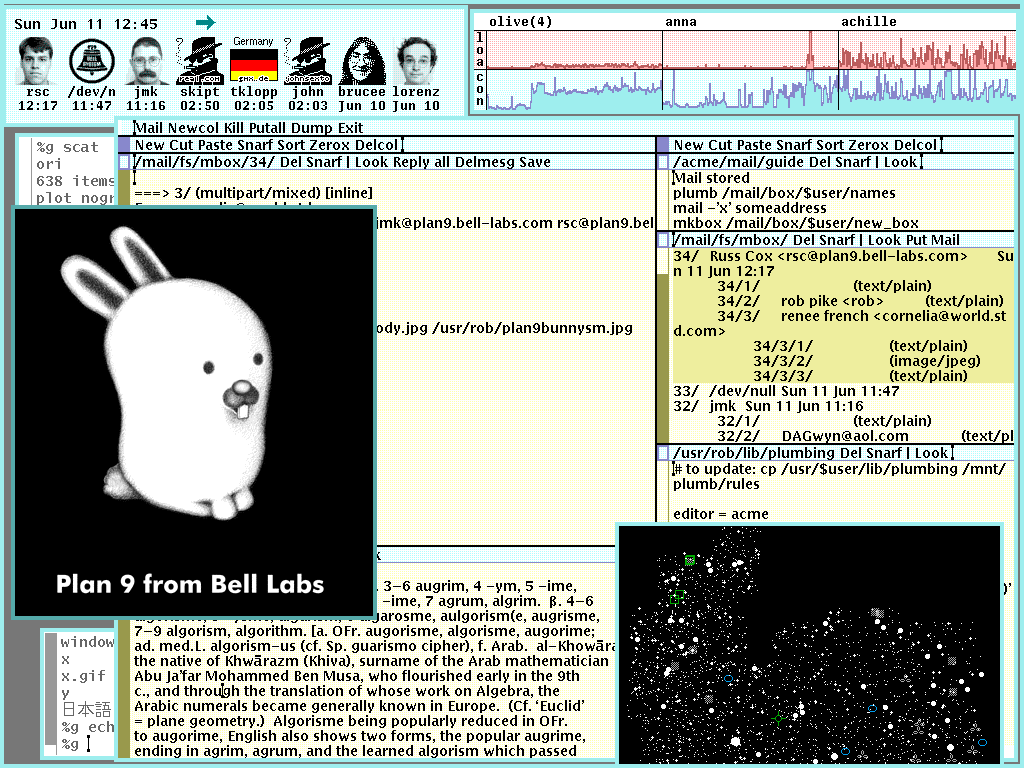
\includegraphics[width=\textwidth]{plan9.png}
                \end{column}
        \end{columns}
\end{frame}

\begin{frame}[label=cc]{Plan9. Кросскомпиляция}
        % http://doc.cat-v.org/plan_9/2nd_edition/papers/comp
        \begin{itemize}
                \item Компиляторы: 2c, 8c, 8al, 8g, 6a, 6c...
                \item Компоновщики: 2l, 8l, 6l...
                \item Первый символ обозначает архитектуру "O"
                \item Компилятор создает объектный файл \texttt{file.<O>}
                \item Объектный файл --- псевдо-ассемблер
                \item Компоновщик присваивает инструкции
                \item \texttt{\% 6c -o test.6 test.c; 6l -o 6.test test.6}
                \item Или вот так: \texttt{\% objtype=amd64 mk}
        \end{itemize}
\end{frame}

\begin{frame}{Архитектуры Plan9 (современные)}
        \begin{columns}[T,onlytextwidth]
                \begin{column}{0.5\textwidth}
                        \begin{itemize}
                                \item \textbf{k}: SPARC
                                \item \textbf{x}: AT\&T DSP3210
                                \item \textbf{v}: be MIPS 3000
                                \item \textbf{q}: PowerPC
                                \item \textbf{0}: le MIPS 3000
                        \end{itemize}
                \end{column}
                \begin{column}{0.5\textwidth}
                        \begin{itemize}
                                \item \textbf{1}: Motorola 68000
                                \item \textbf{2}: Motorola 68040
                                \item \textbf{5}: le ARM
                                \item \textbf{6}: AMD64
                                \item \textbf{7}: ARM64
                                \item \textbf{8}: i386
                        \end{itemize}
                \end{column}
        \end{columns}
\end{frame}

\begin{frame}{Редактор Acme}
        \begin{columns}[T,onlytextwidth]
                \begin{column}{0.44\textwidth}
                        \begin{itemize}
                                \item Для разработчиков
                                \item Автор --- \emph{Роб Пайк}
                                \item Написан на Alef
                                \item Alef = Acme
                                \item 30 лет с нами
                        \end{itemize}
                \end{column}
                \begin{column}{0.56\textwidth}
                        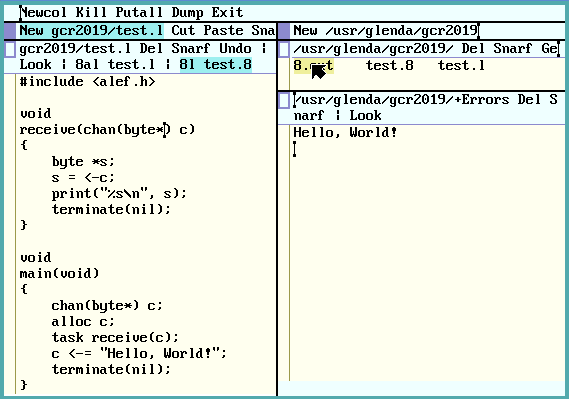
\includegraphics[width=\textwidth]{acme-alef.png}
                \end{column}
        \end{columns}
\end{frame}

\begin{frame}{За несколько лет до этого...}
        \begin{itemize}
                \item 1978 --- \emph{Тони Хоар}. Взаимодействие последовательных процессов
                \item 1982+ --- \emph{Роб Пайк}. Blit, mps, mux
                \item 1985 --- \emph{Лука Карделли} и \emph{Роб Пайк}. Язык Squeak
                \item 1988 --- \emph{Роб Пайк}. Язык Newsqueak. Игрушечные окошки
                \item 1989-2002 --- \emph{Роб Пайк}. Окна 8½, rio
                \item 1989-1995 --- \emph{Фил Винтерботтом}. Язык Alef на основе Newsqueak
        \end{itemize}
\end{frame}

\begin{frame}{Язык Alef}
        \begin{itemize}
                \item Нет сборщика мусора
                \item Частично написан на самом себе (рантайм)
                \item Компилятор создаёт стандартные объекты
                \item Параллельное и конкурентное программирование
                \item Последняя версия --- 1995 год
        \end{itemize}
\end{frame}

\begin{frame}[fragile]{Alef. Каналы}
        \begin{columns}[T,onlytextwidth]
                \begin{column}{0.48\textwidth}
                        \begin{lstlisting}[linebackgroundcolor={\btLstHL{5,11,14}}]
#include        <alef.h>

void receive(chan(byte*) c) {
        byte *s;
        s = <-c;
        print("%s\n", s);
        terminate(nil);
}

void main(void) {
        chan(byte*) c;
        alloc c;
        proc receive(c);
        c <-= "hello world";
        terminate(nil);
}                        \end{lstlisting}
                \end{column}
                \begin{column}{0.48\textwidth}
                        \begin{itemize}
                                \item Синхронные
                                \item Асинхронные
                                \item Всё, как мы любим
                                \item И между процессами
                                \item И между корутинами
                        \end{itemize}
                \end{column}
       \end{columns}
\end{frame}

\begin{frame}[fragile]{Alef. Параллелизм}
        \begin{columns}[T,onlytextwidth]
                \begin{column}{0.48\textwidth}
                        \begin{lstlisting}[linebackgroundcolor={\btLstHL{8,9,11,14}}]
chan(int) a0, a1;

void produce(chan(int) j, int c);

void main(void) {
    int i;
    alloc a0, a1;
    proc produce(a0, '0');
    proc produce(a1, '1');
    for(i = 0; i < 10; i++)
        par {
            a0 <-= i;
            a1 <-= i;
        }
}                       \end{lstlisting}
                \end{column}
                \begin{column}{0.5\textwidth}
                        \texttt{proc}: запуск процесса \\
                        \texttt{par}: параллельный запуск
                \end{column}
       \end{columns}
\end{frame}

\begin{frame}[fragile]{Alef. Хороший пример "par"}
        \begin{lstlisting}[linebackgroundcolor={\btLstHL{7,9,10}}]
active = malloc(BUFSIZE);
passive = malloc(BUFSIZE);

n = decode(fd, active, BUFSIZE);    /* first block */
while(active != nil) {
    par {
        display(active, n);

        if(decode(fd, passive, BUFSIZE) <= 0)
            passive = nil;
    }
    (active, passive) = (passive, active);
}       \end{lstlisting}
\end{frame}

\begin{frame}[fragile]{Alef. Конкурентность}
        \begin{lstlisting}[linewidth=0.75\textwidth,xleftmargin=0.05\textwidth,linebackgroundcolor={\btLstHL{7,9,16}}]
void produce(chan(int) c);

void main(void) {
  int a,i;
  chan (int) c1, c2;
  alloc c1, c2;
  task produce(c1),produce(c2);
  for(i = 0; i < 10 ; i++)
    alt {
        case a =<-c1:
          print("1 -> %d\n",a);
          break;
        case a =<-c2:
          print("2 -> %d\n",a);
          break;
    };
}       \end{lstlisting}
\end{frame}

\begin{frame}{Alef. Планировщик}
        \begin{itemize}
                \item<1-> Процессы (\texttt{proc}):
                \begin{itemize}
                       \item планируются системой
                        \item синхронизируются \textcolor{blue}{rendezvous(2)}
                \end{itemize}
                \item<2-> Корутины (\texttt{task}):
                \begin{itemize}
                        \item переключаются: \texttt{QLock.lock, Rendez.sleep, alt, <-=, <-}
                \end{itemize}
                \item<3-> Коммуникация через каналы
        \end{itemize}
\end{frame}

\begin{frame}[fragile]{Alef. Возврат функций}
        \begin{lstlisting}[basicstyle=\fontsize{14pt}{12}\bf\ttfamily\color{black},linebackgroundcolor={\btLstHL{4,8}}]
int i,j;
float f;

tuple(int, int, float) test(int c) {
        return (c, c+1, (float)c/(float)(c+1));
}

(i, j, f) = test(1);\end{lstlisting}
\end{frame}

\begin{frame}[fragile]{Alef. Обработка ошибок}
        \begin{columns}[T,onlytextwidth]
                \begin{column}{0.38\textwidth}
                        \begin{lstlisting}[basicstyle=\fontsize{14pt}{12}\bf\ttfamily\color{black},linebackgroundcolor={\btLstHL{3,6,11}}]
alloc p;

rescue {
        unalloc p;
        return nil;
}

...

if(error)
        raise;
return p;               \end{lstlisting}
                \end{column}
                \begin{column}{0.58\textwidth}
                        \begin{itemize}
                                \item Блок в контексте функции
                                \item Явный вызов
                                \item Закрытие файлов, unalloc
                        \end{itemize}
                \end{column}
       \end{columns}
\end{frame}

\begin{frame}[fragile]{Alef. Полиморфный тип данных}
        \begin{columns}[T,onlytextwidth]
                \begin{column}{0.48\textwidth}
                        Равнозначная структура:
                        \begin{lstlisting}[linebackgroundcolor={%
                                \btLstHL<1>{3-4}%
                                \btLstHL<2->{}%
                                }]
aggr Polytype
{
        void*   ptr;
        int     tag;
};                      \end{lstlisting}
                \end{column}
                \begin{column}{0.48\textwidth}
                        Особенности:
                        \begin{lstlisting}[linebackgroundcolor={%
                                \btLstHL<1>{}%
                                \btLstHL<2>{1}%
                                \btLstHL<3>{6-8}%
                                \btLstHL<4>{9}%
                                \btLstHL<5>{10}
                                }]
typedef Interface;

Interface a, b, c, d;
int i;

a = (alloc Interface)10;
b = (alloc Interface)"Hello";
d = (alloc Interface)i;
c = a;  /* copy pointer */
d := b; /* copy value */  \end{lstlisting}
                \end{column}
        \end{columns}
\end{frame}

\begin{frame}{Alef. Программирование}
        \begin{itemize}
                \item На Alef не очень хорошая документация
                \item Руководство неплохое, но не полное
                \item Чтобы начать писать, нужно буквально два вечера
        \end{itemize}
\end{frame}

\begin{frame}[fragile]{Alef. Необычный ООП}
        \begin{columns}[T,onlytextwidth]
                \begin{column}{0.58\textwidth}
                        \begin{lstlisting}[linebackgroundcolor={%
                                \btLstHL<1>{1,5}%
                                \btLstHL<2>{2,7}%
                                \btLstHL<3>{3,8-9,12-13}%
                                \btLstHL<4>{6,15}%
                                \btLstHL<5>{7,9}%
                                \btLstHL<6>{8,13}%
                                }]
adt Point {
    int x,y;
    void set(*Point,int,int);
};
adt Circle {
           Point;
    extern int radius;
           void set(*Circle,int,int,int);
    intern int tst(*Circle);
};
...
void
Circle.set(Circle *c, int x, int y, int r)
{
    c->Point.set(x,y);
    c->radius = r;
}                       \end{lstlisting}
                \end{column}
                \begin{column}{0.38\textwidth}
                        \begin{lstlisting}[linebackgroundcolor={%
                                \btLstHL<1->{}%
                                \btLstHL<6>{3}%
                                }]
...
Circle c;
c.set(5,4,3);           \end{lstlisting}
                        \begin{itemize}
                                \item<1-|alert@+>Абстрактный тип
                                \item<2-|alert@+>Поля
                                \item<3-|alert@+>Методы
                                \item<4-|alert@+>Встраивание
                                \item<5-|alert@+>Скрытие
                                \item<6-|alert@+>Передача ссылки
                        \end{itemize}
                \end{column}
        \end{columns}
\end{frame}

\begin{frame}[fragile]{Alef. Дженерики}
                        \begin{itemize}
                                \item<1-|alert@+> Абстрактный тип с параметром
                                \item<2-|alert@2-3> Полиморфный тип и приведение типов
                        \end{itemize}
        \begin{columns}[T,onlytextwidth]
                \begin{column}{0.46\textwidth}
                        \begin{lstlisting}[linebackgroundcolor={%
                                \btLstHL<1>{1}%
                                \btLstHL<2>{7,11}%
                                \btLstHL<3>{8,12}%
                                \btLstHL<4>{7}%
                                \btLstHL<5>{7}%
                                }]
adt Stack[T] {
    extern int  tos;
           T    data[100];
           void push(*Stack, T);
};

Stack[int] bound;
Stack unbound;

/* type casting */
bound.f(3);
unbound.f((alloc T)3);\end{lstlisting}
                \end{column}
                \begin{column}{0.50\textwidth}
                        \begin{lstlisting}[linebackgroundcolor={%
                                \btLstHL<1->{}%
                                \btLstHL<4>{3}%
                                \btLstHL<5>{4,5}%
                                }]
int i, j, k;

i := bound.data[bound.tos];
j = bound.data[bound.tos];
k = bound.data[bound.tos]; /* err */\end{lstlisting}
                        \begin{itemize}
                                \item<4-|alert@4> "\texttt{:=}": без освобождения
                                \item<5-|alert@5> "\texttt{=}": с освобождением
                        \end{itemize}
                \end{column}
        \end{columns}
\end{frame}

\begin{frame}[fragile]{Alef. Biobuf}
        \begin{lstlisting}[basicstyle=\fontsize{14pt}{12}\bf\ttfamily\color{black}]
#include <alef.h>
#include <bio.h>

Biobuf stdout;

void
main(void)
{
        stdout.init(1, OWRITE);
        stdout.print("hello world!\n");
}        \end{lstlisting}
\end{frame}

\begin{frame}{Заброшен и забыт}
        \begin{itemize}
                \item 1995г --- Plan9 2-nd edition
                \item 1995г --- Windows'95
                \item 1995г --- Java
                \item Bell Labs бросается создавать конкурента Java
                \item Plan9 заброшен
                \item Alef прекращает существование
                \begin{itemize}
                        \item Нет сборщика мусора
                        \item Трудно поддерживать
                        \item По слухам, дженерики трудно реализовать со сборщиком мусора
                \end{itemize}
         \end{itemize}
\end{frame}

\begin{frame}{Inferno}
        \begin{columns}[T,onlytextwidth]
                \begin{column}{0.44\textwidth}
                        \begin{flushright}
                        {\small\emph{Земную жизнь пройдя до половины,\\
Я очутился в сумрачном лесу,\\
Утратив правый путь во тьме долины.\\
                        }}
                        \end{flushright}
                        \begin{itemize}
                                \item 1996 --- версия 1.0
                                \item Наследник Plan9
                                \item Новый 9P --- Styx
                                \item Регистровая Dis VM
                        \end{itemize}
                \end{column}
                \begin{column}{0.54\textwidth}
                        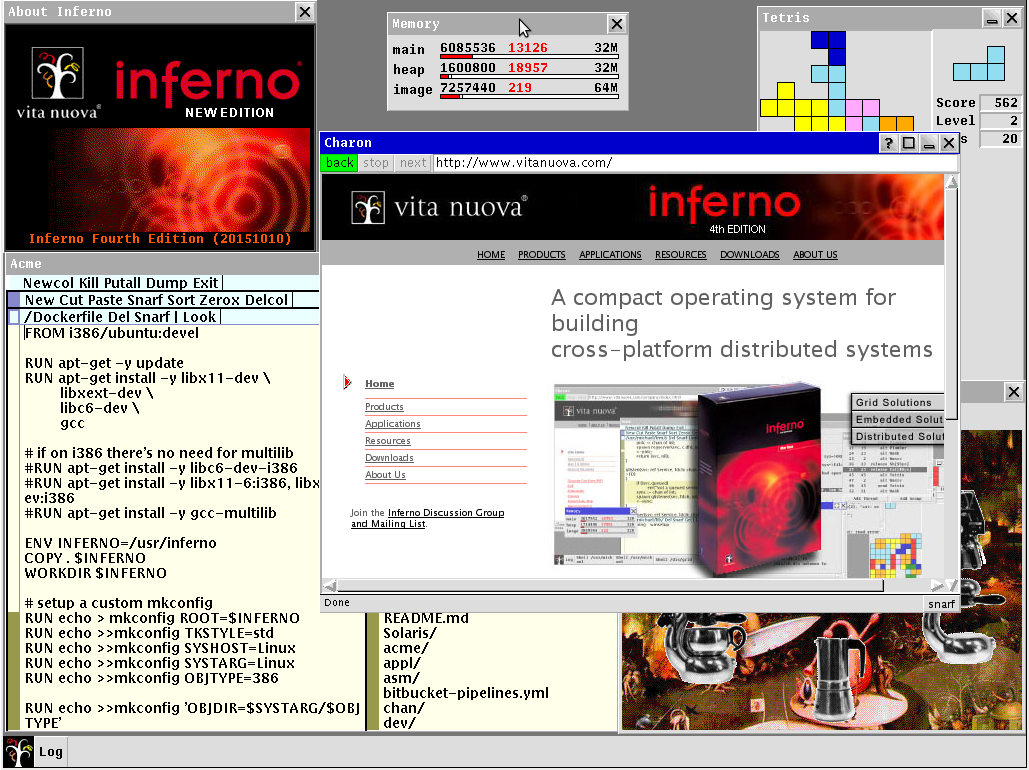
\includegraphics[width=\textwidth]{inferno.png}
                \end{column}
        \end{columns}
\end{frame}

\begin{frame}{Редактор Acme}
        \begin{columns}[T,onlytextwidth]
                \begin{column}{0.42\textwidth}
                        \begin{itemize}
                                \item Для разработчиков
                                \item Автор --- \emph{Роб Пайк}
                                \item Переписан на Limbo
                                \item 30 лет с нами
                        \end{itemize}
                \end{column}
                \begin{column}{0.54\textwidth}
                        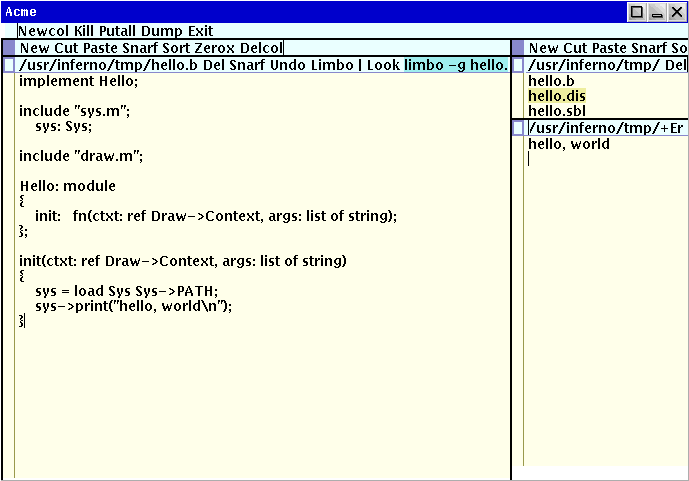
\includegraphics[width=\textwidth]{acme-limbo.png}
                \end{column}
        \end{columns}
\end{frame}

\begin{frame}{Limbo}
        \begin{itemize}
                \item "JIT-ed Newsqueak" \emph{(Роб Пайк, 2007)} % https://youtu.be/hB05UFqOtFA
                \item Сборщик мусора, реализованный в виртуальной машине
                \item Планировщик --- виртуальная машина
                \item Результат --- байткод для виртуальной машины
                \item Только вытесняющие процессы
                \item Идеология модулей
                \item В последнем релизе появились дженерики
        \end{itemize}
        %http://www.vitanuova.com/inferno/papers/addendum.pdf
        %https://github.com/henesy/limbobyexample
        %http://doc.cat-v.org/inferno/4th_edition/release_notes/changes
\end{frame}

\begin{frame}{Limbo. Некоторые замечания}
        \begin{itemize}
                \item Крайне мало документации
                \item Некоторый функционал ограничен
                \item Использовался в промышленных продуктах
                \item Имеет много сохранившегося кода
                \item Работать с кодом Limbo непривычно и сложно
                \item Go --- прямой потомок Limbo? Посмотрим
       \end{itemize}
\end{frame}

\begin{frame}[fragile]{Limbo. Hello, World!}
        \begin{lstlisting}
implement Hello;

include "sys.m";
        sys: Sys;
include "draw.m";

Hello: module
{
        init:   fn(ctxt: ref Draw->Context, argv: list of string);
};

init(ctxt: ref Draw->Context, argv: list of string)
{
        sys = load Sys Sys->PATH;
        sys->print("Hello World\n");
}       \end{lstlisting}
\end{frame}

\begin{frame}[fragile]{Limbo. Примеры синтаксиса}
        %:=, функции с многими, обратная запись не int x, а x int
        %дженерики (2004), нет включения, слайсы, строки, буфер
        % https://powerman.name/Inferno/Limbo.html
        \begin{lstlisting}[basicstyle=\fontsize{12pt}{12}\bf\ttfamily\color{black},linebackgroundcolor={%
                \btLstHL<1>{1}%
                \btLstHL<2>{2-3}%
                \btLstHL<3>{5,6}%
                \btLstHL<4>{8,9}%
                \btLstHL<5>{11}%
                }]
i, j: int;
k := 1;         # int
b := byte 2;    # byte

s: string;      # длина в символах
s1 := s[0:];    # срез

a: array of int;
a = array[10] of int;

myfunc: fn(i, k: int, s: string) : (list of string, int);
        \end{lstlisting}
\end{frame}

\begin{frame}[fragile]{Limbo. Дженерики}
        %http://doc.cat-v.org/inferno/4th_edition/release_notes/changes
        \begin{lstlisting}[basicstyle=\fontsize{12pt}{12}\bf\ttfamily\color{black},linebackgroundcolor={%
                \btLstHL{1,9}%
                }]
reverse[T](l: list of T): list of T
{
        rl: list of T;
        for(; l != nil; l = tl l)
                rl = hd l :: rl;
        return rl;
}

Tree: adt[T] {
    v: T;
    l, r: cyclic ref Tree[T];
};      \end{lstlisting}
\end{frame}

\begin{frame}[fragile]{Limbo. Bufio}
        \begin{lstlisting}[basicstyle=\fontsize{12pt}{12}\bf\ttfamily\color{black},linebackgroundcolor={%
                \btLstHL{6,7}%
                }]
init(nil: ref Draw->Context, nil: list of string)
{
    sys := load Sys Sys->PATH;
    bufio = load Bufio Bufio->PATH;

    bout = bufio->fopen(sys->fildes(1), Bufio->OWRITE);
    bout.puts("Hello World\n");
    
    bout.flush();
}        \end{lstlisting}
\end{frame}

\begin{frame}{Резкий разворот}
        %Alef всё, нужно на чем-то писать Acme, libthread
        \begin{itemize}
                \item Inferno не <<взлетел>> и продан Vita Nuova
                \item Lucent делает новый релиз Plan9 в 2000 году
                %\item На чем-то надо было писать редактор Acme
                \item Библиотека libthread на замену Alef
        \end{itemize}
\end{frame}

\begin{frame}{Редактор Acme}
        \begin{columns}[T,onlytextwidth]
                \begin{column}{0.4\textwidth}
                        \begin{itemize}
                                \item Для разработчиков
                                \item Автор --- \emph{Роб Пайк}
                                \item C и libthread
                                \item 30 лет с нами
                        \end{itemize}
                \end{column}
                \begin{column}{0.6\textwidth}
                        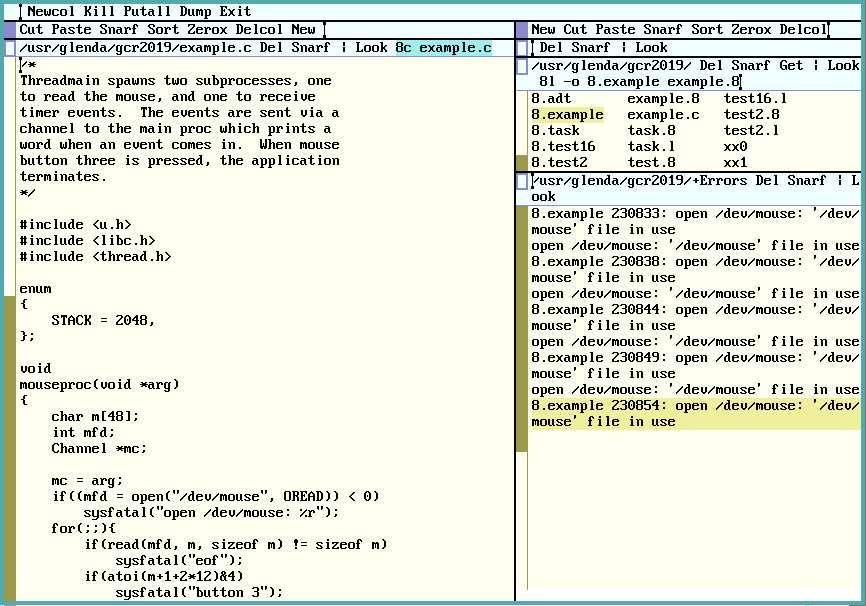
\includegraphics[width=\textwidth]{acme-libthread.png}
                \end{column}
        \end{columns}
\end{frame}

\begin{frame}{libthread}
        % http://man.cat-v.org/plan_9/2/thread
        \begin{itemize}
                \item Написана на C
                \item Работает и с процессами, и с корутинами
                \item Корутины переключаются: \texttt{yield, proccreate, procexec, procexecl, threadexits, alt, send, recv (и основанными на send и recv), qlock, rlock, wlock, rsleep}
                \item Коммуникация через каналы
        \end{itemize}
\end{frame}

\begin{frame}[fragile]{libbio. Подсчет рун}
        \begin{lstlisting}[basicstyle=\fontsize{14pt}{12}\bf\ttfamily\color{black},linebackgroundcolor={%
                \btLstHL{3,6-7}%
                }]
uvlong runecount(Biobuf *f, char *filename) {
    uvlong n;
    Rune r;
    n = 0;

    while((r = Bgetrune(f)) != (Rune)Beof)
        n++;

    print("%10ulld %s\n", n, filename);

    return n;
}        \end{lstlisting}
\end{frame}

\begin{frame}
        \center\textbf{Наши дни}
\end{frame}

\begin{frame}[t]{Вселенная Plan9}
        Конкурентное программирование на примере Newsqueak
        \begin{columns}[T,onlytextwidth]
                \begin{column}{0.46\textwidth}
                        \begin{itemize}
                                \item Март 2007 года. Google
                                \item Newsqueak из 1988
                                \item В сентябре 2007...
                        \end{itemize}
                \end{column}
                \begin{column}{0.52\textwidth}
                        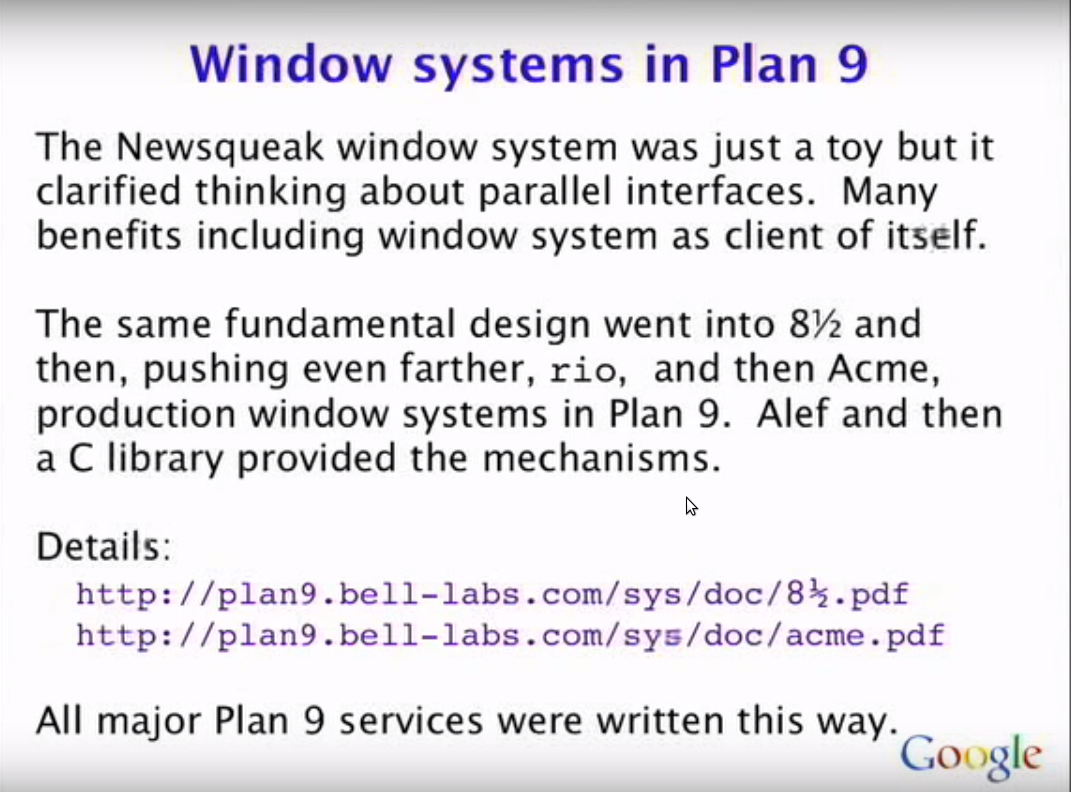
\includegraphics[width=0.82\textwidth]{newsqueak-2017.png}\\
                        \textcolor{blue}{\href{https://youtu.be/hB05UFqOtFA}{https://youtu.be/hB05UFqOtFA}}
                \end{column}
        \end{columns}
\end{frame}

\begin{frame}{Редактор Acme}
        \begin{columns}[T,onlytextwidth]
                \begin{column}{0.42\textwidth}
                        \begin{itemize}
                                \item Для разработчиков
                                \item Автор --- ???
                                \item Переписать на Go
                                \item 30 лет с нами
                        \end{itemize}
                \end{column}
                \begin{column}{0.54\textwidth}
                        
\includegraphics[width=0.82\textwidth]{unclesam.png}
                \end{column}
        \end{columns}
\end{frame}

\begin{frame}{Go}
        % https://go.googlesource.com/go/+/refs/tags/weekly.2009-11-06
        \begin{itemize}
                \item Сентябрь 2007 года --- начало разработки
                \item Первые версии собирались только на Plan9
                \item Из Go, пока он был на C, <<торчали уши>> Plan9
                \item Отказался от процессов и дженериков
                \item Взял ООП, каналы, корутины и кросскомпиляцию
                \item Авторы Go всё знают и хорошо подумали
                \item Если что-то не ясно в Go --- поищите в его истории
                \item Отличный пример --- Go-ассемблер
        \end{itemize}
\end{frame}

\begin{frame}{Использования Go-ассемблера}
        Только если вы \textbf{отлично} представляете, что делаете\\~\\
        \begin{itemize}
                \item Cloudflare CIRCL
                        \begin{itemize}
                                \item \textcolor{blue}{\href{https://blog.cloudflare.com/introducing-circl}{blog.cloudflare.com/introducing-circl/}}
                        \end{itemize}
                \item Шифр <<Кузнечик>> на языке Go
                        \begin{itemize}
                                \item \textcolor{blue}{\href{https://dxdt.ru/2019/02/18/8702/}{dxdt.ru/2019/02/18/8702/}}
                                \item Прямое использование AVX
                        \end{itemize}
        \end{itemize}
\end{frame}

\againframe{cc}

\begin{frame}{Язык ассемблера Go}
        % https://youtu.be/KINIAgRpkDA
        % https://golang.org/doc/asm
        % https://9p.io/sys/doc/asm.html
        \begin{itemize}
                \item Официальный сайт отсылает к Plan9
                \item Это все же не совсем Plan9-ассемблер
                \item Псевдо-ассемблер
                \item Пайк про Go-ассемблер: \textcolor{blue}{\href{https://youtu.be/KINIAgRpkDA}{youtu.be/KINIAgRpkDA}}
                \item Полезные таблицы: \textcolor{blue}{\href{https://quasilyte.dev/blog/post/go-asm-complementary-reference/}{quasilyte.dev/blog/post/go-asm-complementary-reference/}}
                \item Понимание принципов компиляции в Plan9 помогло
        \end{itemize}
\end{frame}

\begin{frame}{Вопросы}
        \center Авторы Go всё знают и хорошо подумали\\Если что-то не ясно в Go --- поищите в его истории
        \vskip2cm
        \center{schors@gmail.com}
\end{frame}

\nocite{*}
\setbeamertemplate{frametitle continuation}{}

\begin{frame}[t]{Ссылки. Plan9}
\printbibliography[keyword={plan9},notkeyword={en}]
\end{frame}

\begin{frame}[t]{Ссылки. Inferno}
\printbibliography[keyword={inferno},notkeyword={en}]
\end{frame}

\begin{frame}[t]{Ссылки. Разное}
\printbibliography[keyword={common},notkeyword={en}]
\end{frame}

\begin{frame}[t]{Ссылки. Ассемблер}
\printbibliography[keyword={asm},notkeyword={en}]
\end{frame}
\end{document}


